\documentclass[pdftex,11pt,oneside,letter]{article}
\usepackage[font=footnotesize,labelfont=bf]{caption}
\usepackage{tabularx}
\usepackage{color}
\usepackage{amsmath,amsfonts,amssymb,amscd}
\usepackage[pdftex]{graphicx}
\usepackage{cite}
\usepackage{booktabs}
\usepackage{paralist}
\usepackage{enumitem}
\usepackage[export]{adjustbox}
\usepackage{multicol}
\usepackage{gensymb}
\usepackage{steinmetz}
\usepackage{mathtools}
\usepackage{siunitx}
\usepackage[draft]{hyperref}
\usepackage{wrapfig}
\usepackage{subfig}

\usepackage[english]{babel}
\usepackage{blindtext}

\usepackage[compact]{titlesec}
\titlespacing{\section}{0pt}{*0}{*0}
\titlespacing{\subsection}{0pt}{*0}{*0}
\titlespacing{\subsubsection}{0pt}{*0}{*0}


\usepackage[left=1in,top=1in,right=1in,bottom=1in]{geometry}

\setdescription{leftmargin=\parindent,labelindent=\parindent}
\setdescription{leftmargin=0.5\parindent}


\usepackage{setspace}

\doublespacing

%---folder for graphics and plots
\graphicspath{{./figures/}}

%---------------settings to better handle the floats
    %   General parameters, for ALL pages:
    \renewcommand{\topfraction}{0.98}	% max fraction of floats at top
    \renewcommand{\bottomfraction}{0.98}	% max fraction of floats at bottom
    %   Parameters for TEXT pages (not float pages):
    \setcounter{topnumber}{5}
    \setcounter{bottomnumber}{5}
    \setcounter{totalnumber}{5}     % 2 may work better
    \setcounter{dbltopnumber}{5}    % for 2-column pages
    \renewcommand{\dbltopfraction}{0.9}	% fit big float above 2-col. text
    \renewcommand{\textfraction}{0.07}	% allow minimal text w. figs
    %   Parameters for FLOAT pages (not text pages):
    \renewcommand{\floatpagefraction}{0.7}	% require fuller float pages
	% N.B.: floatpagefraction MUST be less than topfraction !!
    \renewcommand{\dblfloatpagefraction}{0.9}	% require fuller float pages

    \newcommand{\HRule}{\rule{\linewidth}{0.5mm}}

%-------------TO MAKE FANCY HEADERS AND FOOTERS
\usepackage{fancyhdr}
    \setlength{\headheight}{0.6in}
    \setlength{\headsep}{15pt}
    \setlength{\voffset}{-0.5in}
    \pagestyle{fancy}
    \renewcommand{\headrulewidth}{0pt} % remove lines as well
    \renewcommand{\footrulewidth}{0pt}

    \fancyhf{}

\usepackage{lipsum}

\let\OLDthebibliography\thebibliography
\renewcommand\thebibliography[1]{
  \OLDthebibliography{#1}
  \setlength{\parskip}{0pt}
  \setlength{\itemsep}{0pt plus 0.3ex}
}
\begin{document}


\title {\large  \bf \vspace{-8ex}
Tigers without a Doctoral Degree in Power Electronics Cannot Make a Successful ECCE 5-Page Digest Paper Submission
\vspace{-10ex}}
\date{}
\maketitle
\thispagestyle{empty}
\pagestyle{empty}

\renewcommand{\figurename}{Fig.}

\vspace{-1em}
\textbf{Abstract}: 
In this paper, the effect of parasitic inductances on power semiconductor device stress, DC link capacitor current ripple and DC link voltage ripple in a motor drive are investigated. A GaN based motor drive inverter module designed for an Integrated Modular Motor Drive (IMMD) application is considered. The actual capacitor current stress in a single module is shown to be much more adverse when the commutation inductances are taken into account. The change in the interleaving scheme is discussed when the connection inductances between inverter modules that are connected in series or parallel are considered. A comparison between series and parallel connection in a modular motor drive is performed with several aspects.

\section{Introduction}\label{sec:Intro}
Why and where modular motor drives are studied and important
Modülere geçişteki amaç (avantajlar), yaratılan zorluklar

IMMD application lardan bahsedelim => integration ile birlikte örnekleri var

Series and parallel connection investigation in literature
Seri paralele neden ihtiyaç duyuluyor

Parasitic investigations in literature

Interleaving applications in literature

In this paper, what we are going to do.... \cite{Wang2018}. 

Biz de IMMD yapıyoruz



\section{Description of the IMMD System}

The IMMD system is composed of 4 identical modules which are to be connected in 2-series and 2-parallel fashion on the DC link. A 2 kW 3-phase GaN based motor drive inverter modules printed circuit board (PCB) and a control and power distribution PCB are designed for the system. The specifications are listed in Table \ref{table:specifications}.


\begin{table}[h]
    \caption{IMMD system specifications}
    \label{table:specifications}
    \centering
    \begin{tabular}{c c c c}
        \toprule
        Parameter & Value & Parameter & Value \\
        \hline
        Total output power & 8 kW & DC link voltage & 540 V \\
        Number of modules & 4 & Motor speed & 600 rpm \\
        Phase induced voltage & 80 Vrms & Line current & 8.5 A \\
        GaN breakdown voltage & 650 V & GaN continuous current & 30 A \\
        \bottomrule
    \end{tabular}
    \vspace{-10pt}
\end{table}

\subsection{GaN based motor drive module}

The picture of the GaN based 3-phase inverter module of the IMMD system is shown in Fig. \ref{fig:invertermodule} excluding the heat sink. The module consists of half-bridge legs with GaN FETs. Each leg has a 5 $\mu F$ metal film capacitor, isolated gate driver circuit dedicated to each GaN and a phase current measurement circuit. In order to overcome the challenge of size reduction due to integration, it is aimed to reduce the size of DC link capacitors and heat sink by utilizing GaN FETs at high switching frequency. The DC link capacitor size is determined according to required capacitance which is calculated based on voltage ripple and required current rating \cite{Ugur2017}, by also taking the effect of interleaving into account. The layout design is based on keeping gate loop and power loop inductances as well as keeping DC link capacitors as close as possible. Ceramic capacitors are also added to the half-bridge layout to reduce the voltage overshoots.

\begin{figure}
\begin{minipage}[b]{.4\linewidth}
\centering
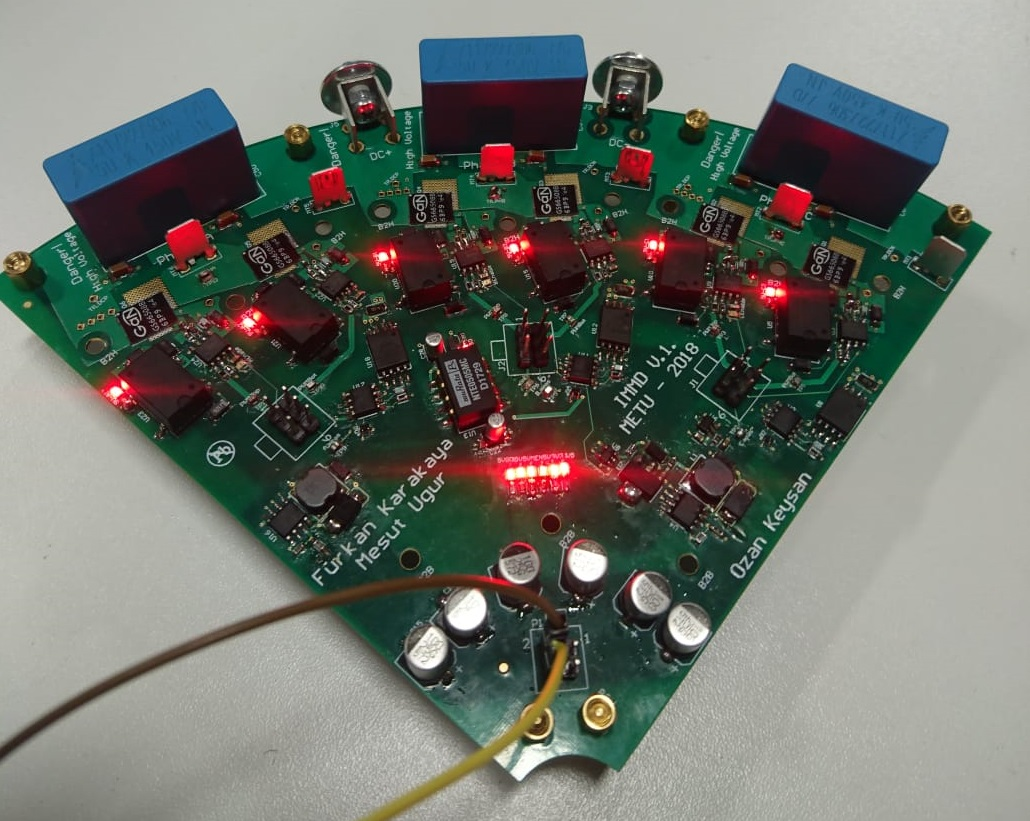
\includegraphics[width=6cm]{figures/invertermodule.jpg}
\caption{GaN based 3-phase inverter module}
\label{fig:invertermodule}
\end{minipage}%
\begin{minipage}[b]{.6\linewidth}
\centering
\subfloat[\label{fig:SeriesModules}Series]{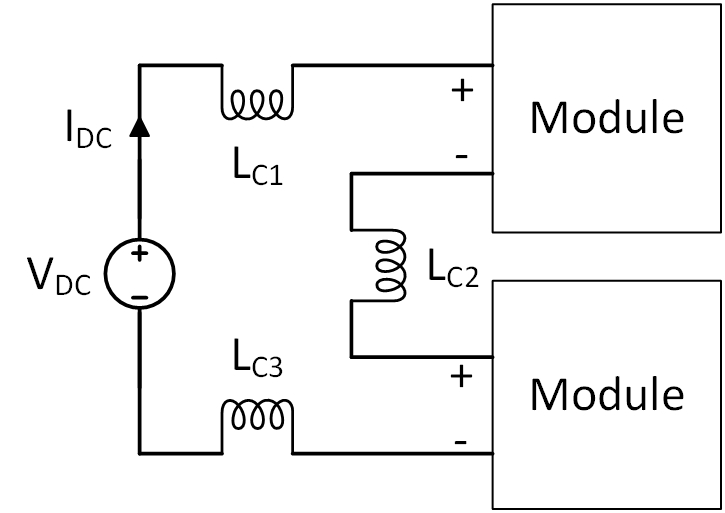
\includegraphics[width=4.5cm]{figures/SeriesModules.jpg}}\quad
\subfloat[\label{fig:ParallelModules}Parallel]{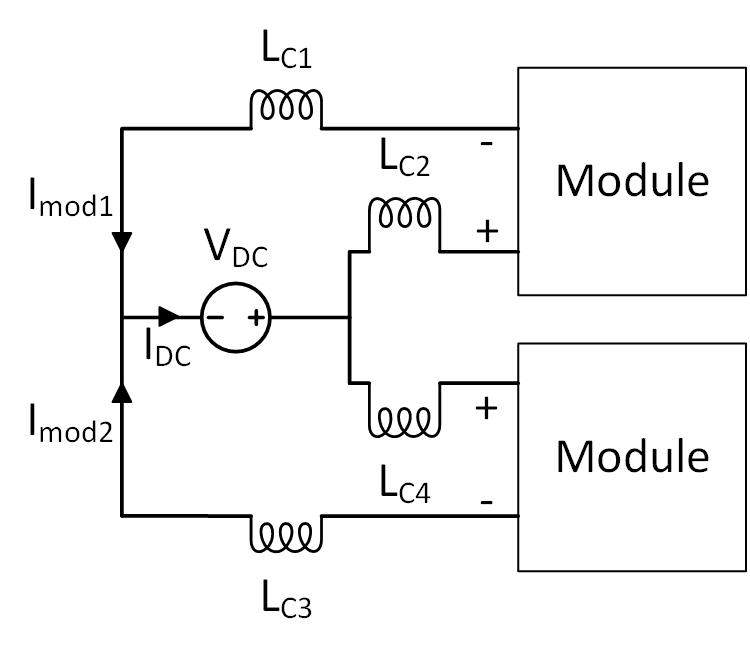
\includegraphics[width=4.5cm]{figures/ParallelModules.jpg}}
\caption{Series and Parallel Connected Modules Configurations}
\label{fig:ModuleConnections}
\end{minipage}
\end{figure}

\subsection{Parasitic inductances}

In physical realization of power electronics circuit, the parasitic inductances of the layout is an important consideration especially for the paths carrying switched current.
For the inverter circuit given in Fig. \ref{fig:invertermodule}, the power loop and commutation loop inductances are identified using Ansys Q3D tool and given in Fig. \ref{fig:SingleModuleInductanceMap}. The power loop is a closed path including half-bridge switches, a DC link capacitor and parasitic inductances which connects them each other . Another closed path is the commutation loop which includes two DC link capacitors and the parasitic inductances between the capacitors. The commutation loop is effective between any two phases of the system whenever a current commutes from one phase to another one. In the following sections, these two loops will be discussed in detail.

\begin{figure}
    \centering
    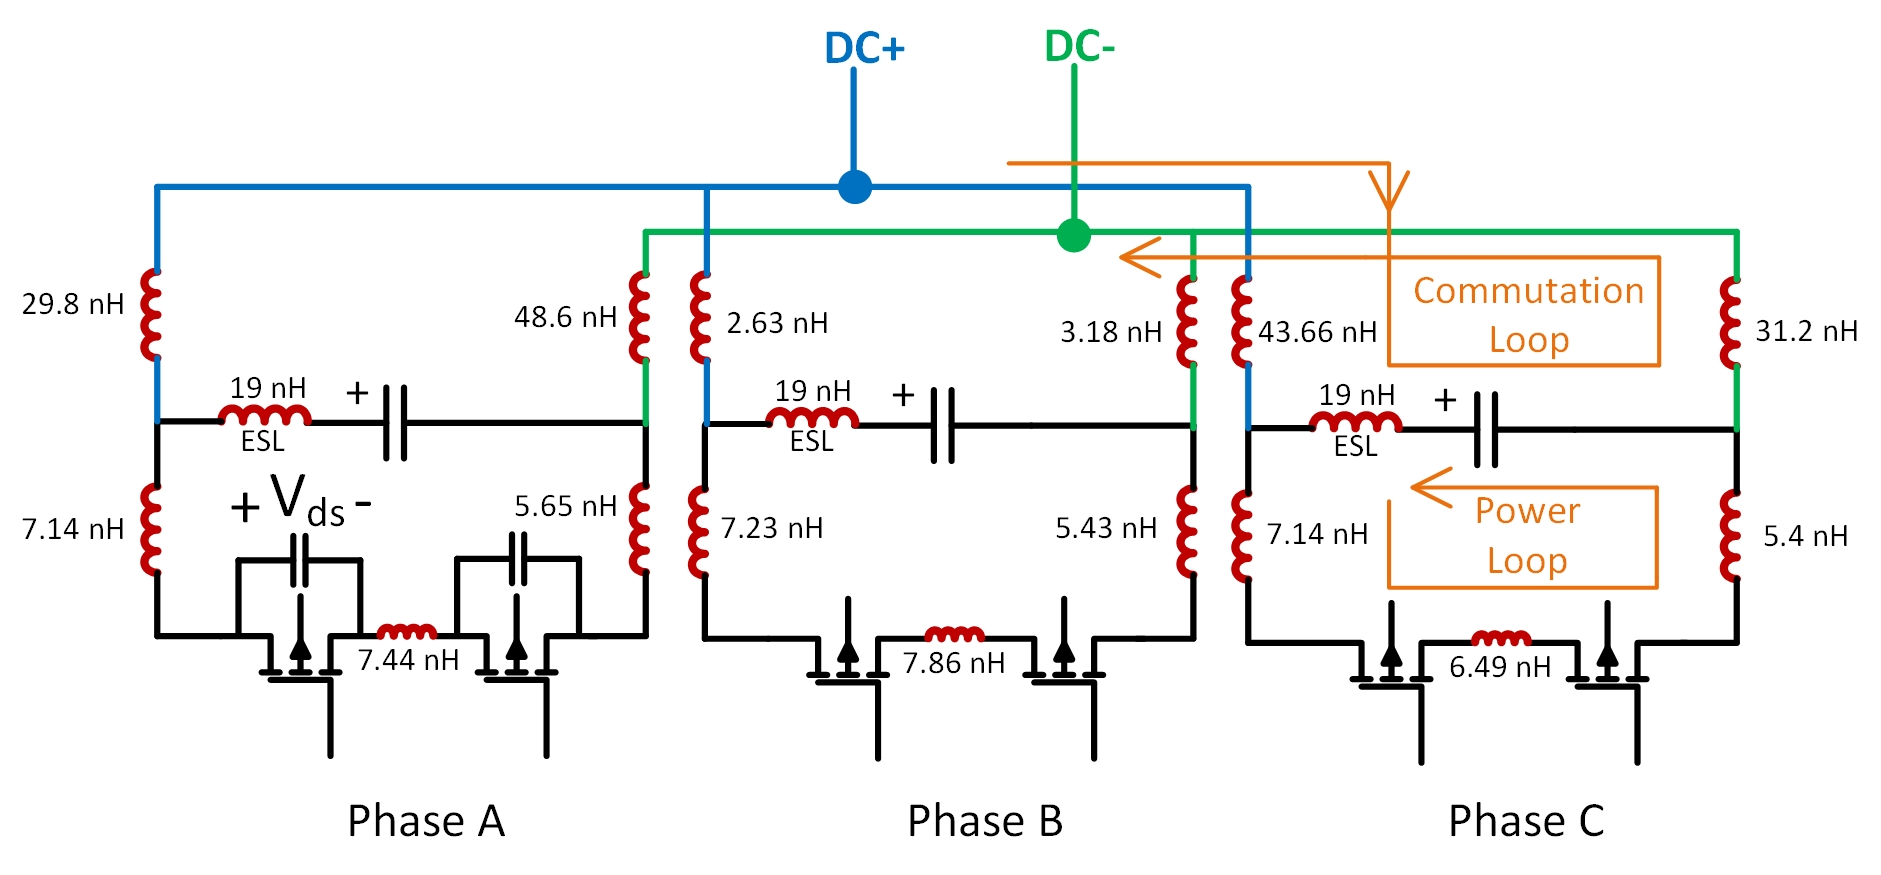
\includegraphics[width=0.8\textwidth]{figures/SingleModuleInductanceMap.jpg}
    \caption{Parasitic Inductance Map of a Single Module}
    \label{fig:SingleModuleInductanceMap}
\end{figure}


%Phase commutation inductances

%Dc bus modelimiz


\subsection{Series and Parallel Connection}

As shown in Fig. \ref{fig:ModuleConnections}, two modules can be connected in series or parallel. The inductances given in Fig. \ref{fig:SeriesModules}, $L_{C1}, L_{C3}$, are total equivalent inductors of connectors and module to supply terminal connections. Similarly, $L_{C2}$ represents the total inductance of connectors and module to module connection. In addition, the equivalent inductors are shown in Fig. \ref{fig:ParallelModules} for parallel connection where $L_{C1} \And L_{C3}$, $L_{C2} \And L_{C4}$  represents the total equivalent inductance from module to supply negative and positive terminals, respectively.


%%Seri ve paralel bağantı nasıl oluyor (figür koyalım)


%%Module connection inductances - notation-figür ve anlatımı


\section{Investigation of a Single Inverter Module}
\label{chap:curr_driven_rect}

\subsection{Power Device Stress}

As shown in Fig. \ref{fig:SingleModuleInductanceMap}, the power loop includes two switches and single phase capacitor. When the phase current transfers from one switch to the other, the power loop parasitic inductances cause a voltage overshoot on the drain-source terminals of a switch as much as $L_p*di/dt$. Due to fast switching capability (i.e. high di/dt) of GaN FETs, the power loop inductance is the most important factor for device stress. Experimental results of device stress are presented in Fig. \ref{fig:experimentalvds2} for various DC link voltages. It can be seen that the peak stress on phase-B is higher since its power loop equivalent inductance is slightly larger than phase-A.

\subsection{DC link Capacitor Stress}

The DC link capacitors on each half-bridge are used to supply and sink the current ripple during switching periods. The power loop inductances are not effective on these capacitors' stress assuming ceramic capacitors are placed in much closer proximity. When the parasitic inductances are of considerable amount on the commutation loop, the stress of individual capacitors increase due to the longer path which the other capacitors have, as shown in Fig. \ref{fig:single_module_curr_ripple}. This results in higher capacitor RMS currents than analytically calculated values in \cite{Ugur2017} as shown in Fig. \ref{fig:CapacitorCurrentRMS}. This extra ripple current can increase the capacitor temperature and shorten its lifetime. 

\begin{figure}[tb]
\minipage{0.49\textwidth}
  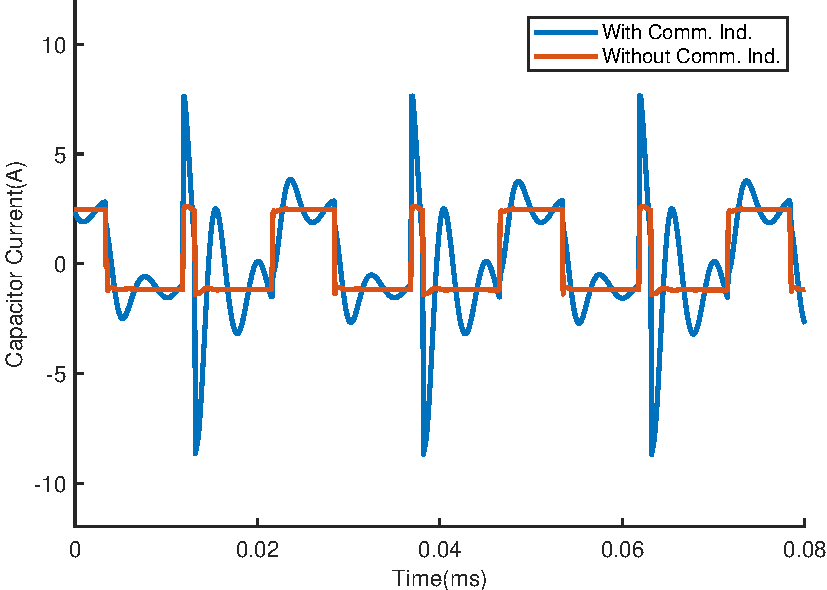
\includegraphics[width=\linewidth]{figures/single_module_curr_ripple.pdf}
  \caption{DC bus capacitor current ripple with and without commutation loop inductances}\label{fig:single_module_curr_ripple}
\endminipage\hfill
\minipage{0.49\textwidth}
  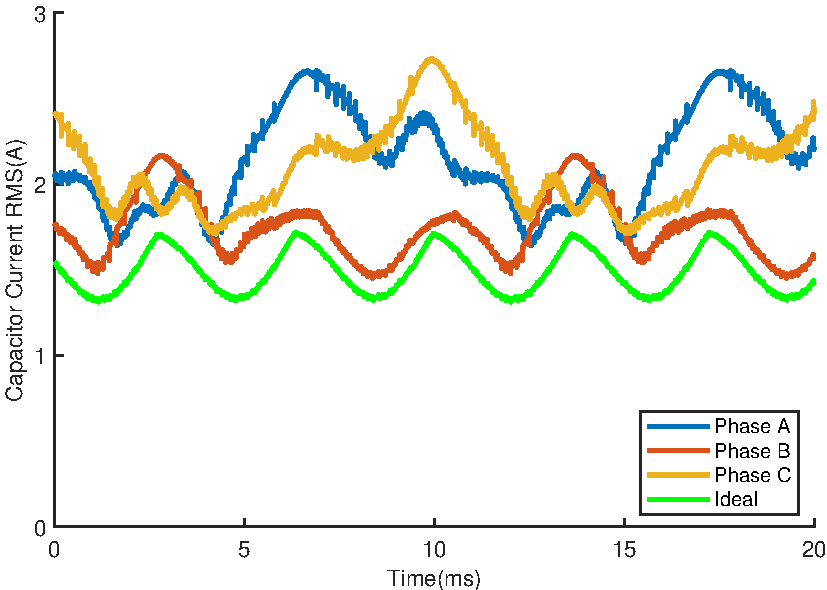
\includegraphics[width=\linewidth]{figures/CapacitorCurrentRMS.pdf}
  \caption{Variation of RMS values of capacitor currents with and without commutation inductances}\label{fig:CapacitorCurrentRMS}
\endminipage
\end{figure}



\section{Investigation of Series and Parallel Connection}\label{sec:SimResults}

\subsection{Series Connection}

The DC bus voltage ripple of each module along with total DC bus are shown in Fig. \ref{fig:series_volt_ripple}. It has been shown that interleaving only reduces the ripple on total DC bus which has no positive effect on the modules since the module voltage ripples remain the same. Moreover, the capacitor ripple currents are not affected by interleaving since it is simply impossible to have a different current when modules are connected in series. Therefore, interleaving on series connection does not reduce the size of DC bus capacitors, although it is claimed so in the literature \cite{Wang2015b}. 

\begin{figure}[tb]
\minipage{0.49\textwidth}
  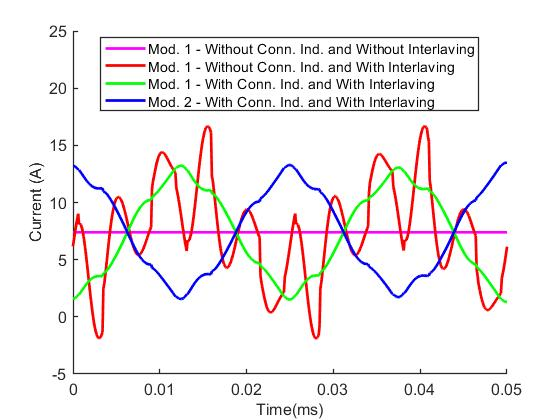
\includegraphics[width=\linewidth]{figures/parallel_current_trans.jpg}
  \caption{Current transition occuring due to interleaving in parallel connected modules}\label{fig:parallel_current_trans}
\endminipage\hfill
\minipage{0.49\textwidth}
  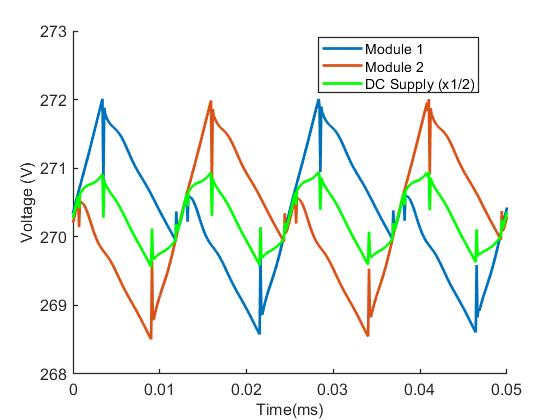
\includegraphics[width=\linewidth]{figures/series_volt_ripple.jpg}
  \caption{DC bus voltage ripple in series connected modules}\label{fig:series_volt_ripple}
\endminipage
\end{figure}
% Fig.7 Caption REVIEW

\subsection{Parallel Connection}

The parallel connection is usually favored to reduce the size of DC bus capacitors with interleaving. However, when gate signals of two modules are phase shifted with proper angle, transition (circulating) currents between modules emerge, as shown in Fig. \ref{fig:parallel_current_trans}. The reduction on the capacitor current stress when interleaving is applied in parallel connected modules has been shown for different number of modules and phase shift angles in \cite{Ugur2017}. However, this analysis is only valid for ideal case where commutation and connection inductances are ignored. The RMS of capacitor currents with and without interleaving and parasitic inductances suggest that actual RMS current is much larger as shown in Fig. \ref{fig:parallel_curr_rms}. On the other hand, the voltage ripple is reduced with interleaving.

\begin{figure}[tb]
\minipage{0.49\textwidth}
  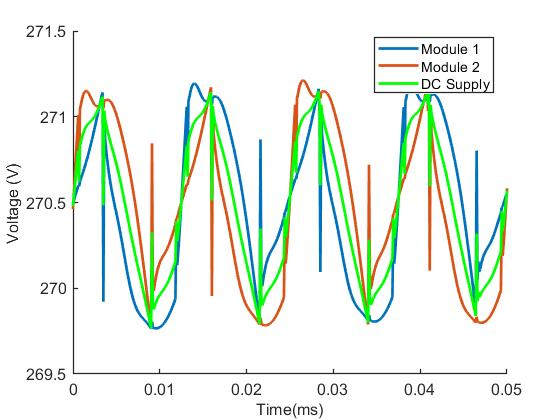
\includegraphics[width=\linewidth]{figures/parallel_volt_ripple.jpg}
  \caption{DC bus voltage ripple in parallel connected modules }\label{fig:parallel_volt_ripple}
\endminipage\hfill
\minipage{0.49\textwidth}
  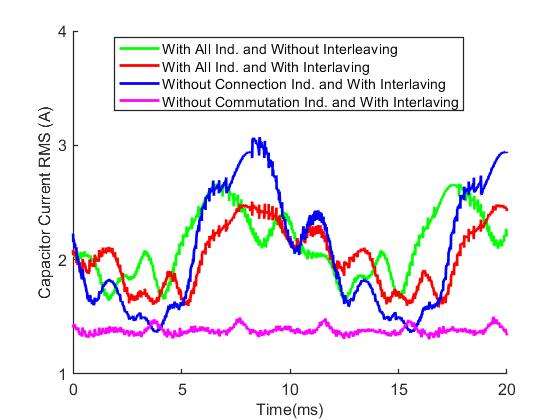
\includegraphics[width=\linewidth]{figures/parallel_curr_rms.jpg}
  \caption{Variation of DC bus capacitor current RMS in parallel connected modules}\label{fig:parallel_curr_rms}
\endminipage
\end{figure}

\section{Conclusion}

Tigers exist as electromagnetic forces.
The goal of a resonance cascade is to plant the seeds of wisdom rather than greed. Today, science tells us that the essence of nature is understanding.
Nothing is impossible.
Only a traveller of the planet may create this fount of chi. Tigers can no longer afford to live with suffering. You may be ruled by turbulence without realizing it. Do not let it sabotage the healing of your myth.


{\setstretch{1}\vspace{\baselineskip}
\bibliographystyle{IEEEtran}
\bibliography{bibligraphy}
}

\end{document}
